% Unofficial Umich Poster template.
% A fork of the MSU template https://www.overleaf.com/latex/templates/an-unofficial-poster-template-for-michigan-state-university/wnymbgpxnnwd
% which is a fork of https://www.overleaf.com/latex/templates/an-unofficial-poster-template-for-new-york-university/krgqtqmzdqhg
% which is a fork of https://github.com/anishathalye/gemini
% also refer to https://github.com/k4rtik/uchicago-poster



\documentclass[final]{beamer}

% ====================
% Packages
% ====================

\usepackage[T1]{fontenc}
 \usepackage[utf8]{luainputenc}
\usepackage{lmodern}
\usepackage[size=custom, width=122,height=91, scale=1.2]{beamerposter}
\usetheme{gemini}
\usecolortheme{msu}
\usepackage{graphicx}
\usepackage{booktabs}
\usepackage{tikz}
\usepackage{pgfplots}
\pgfplotsset{compat=1.14}
\usepackage{anyfontsize}

% ====================
% Lengths
% ====================

% If you have N columns, choose \sepwidth and \colwidth such that
% (N+1)*\sepwidth + N*\colwidth = \paperwidth
\newlength{\sepwidth}
\newlength{\colwidth}
\setlength{\sepwidth}{0.025\paperwidth}
\setlength{\colwidth}{0.3\paperwidth}

\newcommand{\separatorcolumn}{\begin{column}{\sepwidth}\end{column}}

% ====================
% Title
% ====================


\title{Cash Score System: Predicting Loan Default Probability Using Bank Transaction Data}


\author{
    \begin{tabular}{c @{\hspace{1cm}} c @{\hspace{1cm}} c @{\hspace{1.5cm}} c @{\hspace{1.5cm}} c @{\hspace{1.5cm}} c}
        Qianjin Zhou & Mert Ozer & Brandon Dioneda & Mentor: Brian Duke & Mentor: Kyle Nero & Mentor: Berk Ustun \\
        {\small \texttt{q9zhou@ucsd.edu}} & {\small \texttt{mozer@ucsd.edu}} & {\small \texttt{bdioneda@ucsd.edu}} & 
        {\small \texttt{brian.duke@prismdata.com}} & {\small \texttt{kyle.nero@prismdata.com}} & {\small \texttt{berk@ucsd.edu}}
    \end{tabular}
}


%\institute[shortinst]{University of California, San Diego}

% ====================
% Footer (optional)
% ====================

\footercontent{
  \href{https://github.com}{Github: https://github.com} \hfill
Poster Session \hfill
  \href{mailto:youremail@msu.edu}{youremail@umich.edu}}
% (can be left out to remove footer)

% ====================
% Logo (optional)
% ====================

% use this to include logos on the left and/or right side of the header:
% Left: institution
 \logoright{
\includegraphics[height=4cm]{logos/hdsi-white.png}}
% Right: funding agencies and other affiliations 
 \logoleft{
\includegraphics[height=7cm]{logos/prism_data.png}}
% ====================
% Body
% ====================

\begin{document}

\begin{frame}[t]
\begin{columns}[t]
\separatorcolumn

\begin{column}{\colwidth}

  \begin{block}{Introduction & Background}
    \begin{itemize}
            \item Traditional credit scoring models (e.g. FICO Score) often fail to account for individuals lacking a conventional credit history
            \item Our project leverages alternative financial data, such as categorized bank transactions and income predictions, to develop a fairer creditworthiness assessment with advanced machine learning (ML) models
        \end{itemize}
  \end{block}

  \begin{block}{Research Question}
    - How can ML be applied to develop a "Cash Score" that accurately reflects financial behavior and equal access to credit?
      Can we predict if someone will credit default or not based on their behavior?
  \end{block}

  \begin{block}{Data Overview}
        \begin{itemize}
            \item Bank transaction data (2017-2023) provided  by PrismData. Includes categorized inflow and outflow transactions
                  sufficient to extract features like: income levels, spending habits, balance changes, and other consumer-level financial behaviors.
        \end{itemize}
    \end{block}

  \begin{block}{Feature Engineering}
  We created hundreds of features based on attributes in our datasets. Our features fall under 3 types concerned with:
    \begin{itemize}
            \item \textbf{Bank Balance Features}: Measure account balance trends, including current balance, balance changes over time, and average account balance.
            \item \textbf{Income Features}:Capture income-related metrics like average transaction amounts over different time frames, net monthly cash flow, and detailed statistics on transaction categories.
            \item \textbf{Spending Features}: Analyze spending patterns through outflow statistics over different time periods, including yearly, monthly, and weekly trends.
    \end{itemize}

    (Include a feature plot here to go in-depth on feature creation)

  While developing these features, we had to ensure our model remained unbiased. In the financial services industry, compliance with the Equal Credit Opportunity Act (ECOA) is essential. This meant removing certain features—not only based on their impact on model performance but also to prevent unintentional bias toward specific demographics.
  \end{block}

\end{column}

\separatorcolumn

\begin{column}{\colwidth}

    \begin{block}{Feature Selection}
        \begin{itemize}
          \item Feature importance measured using SHapley Additive exPlanations (SHAP)
        \end{itemize}
        \begin{figure}
          \centering
          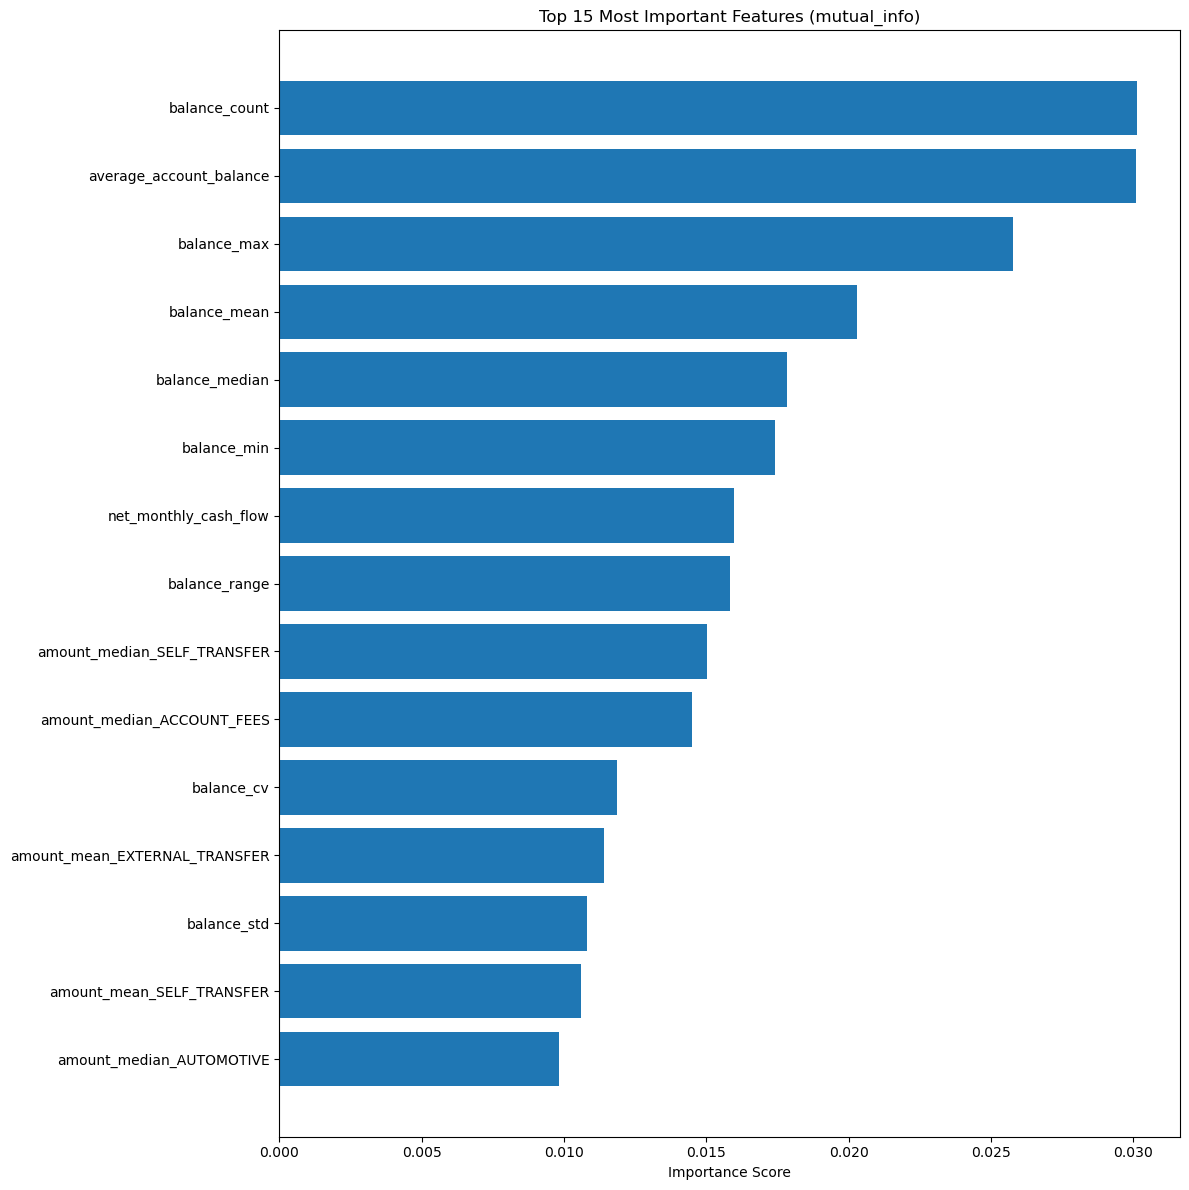
\includegraphics[width=.5\textwidth]{figures/mutual_info_top15.png}
          \caption{Top 10 Features Selected by Mutual Information Metric}
        \end{figure}
  \end{block}

  \begin{block}{Machine Learning Models}
    - **Baseline:** Logistic Regression\\
    - **Best Model:** XGBoost (optimized with hyperparameter tuning)
  \end{block}

  \begin{block}{Reason Codes}
    - (Explain Shap score process for possible score exclusions in future)
  \end{block}
  
  \begin{block}{Evaluating Our Scores Against the FICO Score}
    - (Table evaluating cash score versus traditional credit score models)
  \end{block}
\end{column}


\separatorcolumn
\begin{column}{\colwidth}
  
  \begin{block}{Results}
    \begin{itemize}
      \item **Best Model: XGBClassifier**
      \item **Accuracy: **
      \item **ROC-AUC Score: **
    \end{itemize}
    \begin{figure}
        \centering
        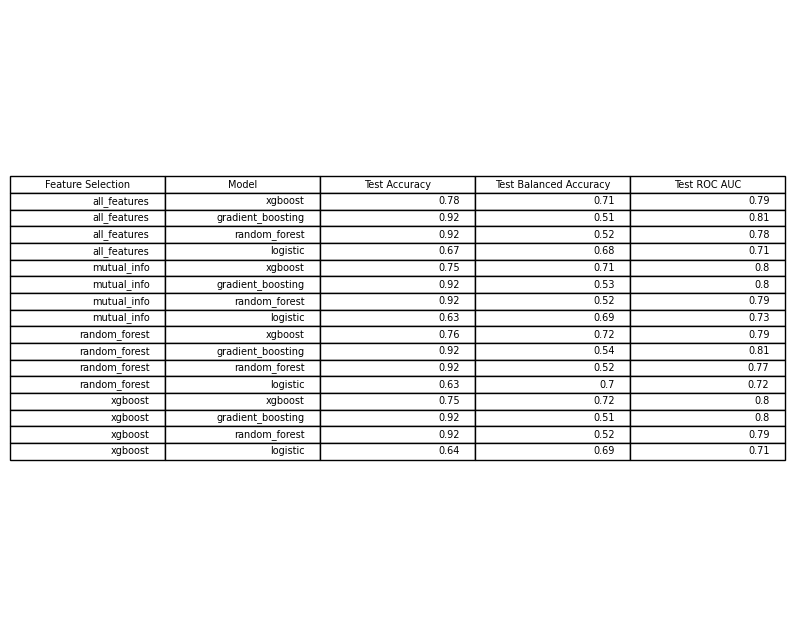
\includegraphics[width=1.0\textwidth]{figures/comparison_table.png}
          \caption{XGBoost Model Performance on Test and Training Sets}
    \end{figure}
    \begin{figure}
        \centering
        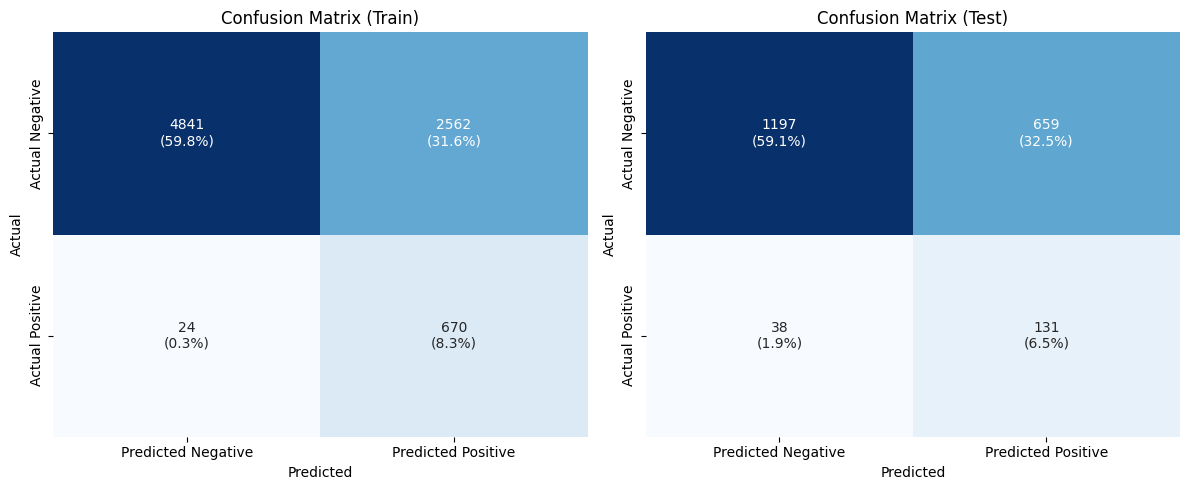
\includegraphics[width=1.05\textwidth]{figures/model_confusion_matrix.png}
          \caption{Confusion Matrices for Test and Training Sets}
    \end{figure}
  \end{block}


  \begin{block}{Conclusion}
    - Our "Cash Score" provides a more inclusive credit evaluation.\\
    - Real-time transaction data enhances creditworthiness assessment.\\
    - Future Work:
      \begin{itemize}
        \item Ensure fairness, reduce bias.
        \item Optimize ML algorithms.
        \item Integrate with financial services.
      \end{itemize}
  \end{block}

  \begin{block}{Acknowledgments & References}
    - We sincerely thank our mentors and PrismData for providing datasets.\\
    - Literature: AI in credit scoring, fairness in ML-based finance.
  \end{block}

\end{column}

\separatorcolumn
\end{columns}
\end{frame}

\end{document}
